%\subsection{Physics of Magnetostriction}
%

This section will talk about Magnetostriction and the physics involved in it. 

Unpaired electrons in the valence shell, or unbalanced spins, can produce significant magnetism in an atom.  However, these electrons are used in bonding when forming a solid making their contribution to magnetism in a solid is negligible\cite{Breu2008}.  The preserved magnetic moments in solids are more characteristic of an element’s ionic electron configuration (Fe{$^{3+}$} rather than Fe) or with sufficient bonding electrons added to complete the shell.  The only groups of elements in the periodic table which exhibit magnetic moments in solids are those in which the unbalanced electron populations occur in an inner shell, namely the transition metals (3\textit{d}, 4\textit{d}, and 5\textit{d}), rare earths (4\textit{f}), and actinides (5\textit{f}).  It is clear that the more tightly bound an unfilled orbital shell is, the less the unpaired electrons will have to do with bonding and the more they will contribute to magnetism.  This is why we see very strong magnetic responses in rare earth materials which use 6\textit{s} and 5\textit{d} shells for bonding before using the very tightly bound 4\textit{f} shell electrons.  The 3\textit{d} electrons in transition metals are less tightly bound to the nucleus, and sometimes 3\textit{d} electrons are used for bonding.  \\

\begin{figure}[h] 
	\centering
	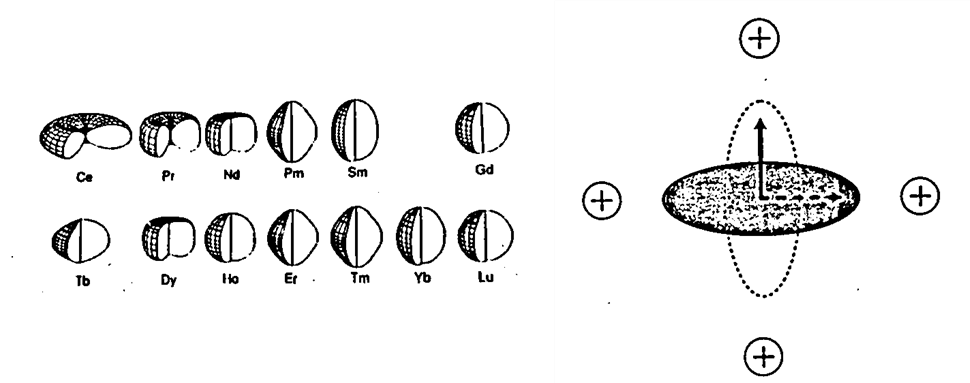
\includegraphics[trim=0pt 10pt 0pt 0pt,scale=1.0]{electron_cloud_density}
	\caption{(a) 4f electron charge cloud densities for a number of rare earth elements. (b) Schematic of oblate 4f charge density of a rare earth element with + nearest neighbors, such as Tb, rotating in a magnetic field. \cite{Engdahl1999} 
	}
	\label{fig:electron_cloud_density}		
\end{figure}

Magneto-elasticity is the coupling between a material’s classical properties of elasticity and strain and the quantum mechanical and relativistic phenomena of magnetism.  When a spin imbalance occurs, electrons can order in such a way that the net magnetic moment points in a particular direction which lowers the crystal symmetry and produces new properties, like magnetostriction.\cite{Breu2008} This coupling between magnetism and elasticity derives from the large contribution of the spin moment to the magnetic moment.  Hence, coupling occurs if there is a strong coupling between the \textit{direction} of the atom’s spin moment and the \textit{orientation} of its anisotropically shaped electron charge cloud, as seen in Figure 1a.  This coupling that exists at the individual electron level is called “spin-orbit coupling,” and since it derives from relativistic aspects of the electron motion, it is one of the smallest energies used to describe the state of an atom.  It is easiest to see this coupling in rare earth elements where the spin directions of rapidly moving 4\textit{f} electrons are strongly coupled to the orientation of their orbits.  This individual electron spin-orbit coupling leads to strong coupling between the total spin moment and the total electron density.  Thus, in rare earth elements the spin moment can be envisioned as rigidly attached to the anisotropically shaped electron charge cloud.  We can now define magnetic anisotropy as the tendency of a magnetic moment to point in a specific crystalline direction, the easy magnetization direction, because of the electrical attraction/repulsion between the rotating electronic charge cloud and neighboring charged ions, as seen in Figure 1b.  It is important to note that 3d electrons obey the same magnetoelastic trends, but with a factor of ten less for spin-orbit coupling.\cite{Engdahl1999}

%testasdasdasasdasdas
%test again
%\subsection{Materials for Magnetostriction}\label{magnetostrict-materials}
%
	
This section talks about commercial magnetostrictive materials, what alternatives are available, why we study them, and what we can do with them. 

\begin{figure}[h] 
	\centering
	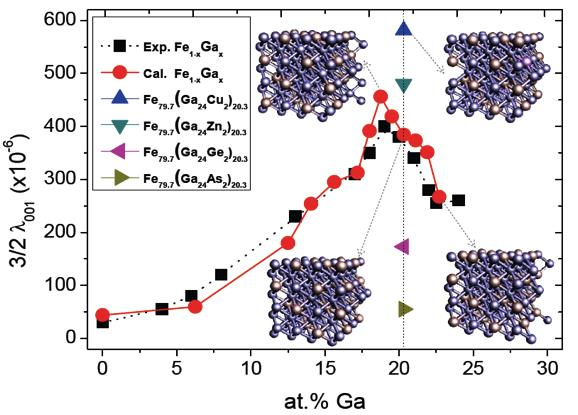
\includegraphics[trim=0pt 10pt 0pt 0pt,scale=1.5]{galfenol-composition-constant}
	\caption{Calculated tetragonal magnetostriction constant (3/2)$\lambda_{001}$ (red circles) and experimental data taken at room temperature (black squares at different Ga concentrations). Triangles show results of four ternary alloys with addition of Cu, Zn, Ge and As. %Insets give the crystal structures with purple and red balls for Fe and Ga atoms, respectively.%
	}
	\label{fig:galfenol-composition-constant}		
\end{figure}

Magnetostriction \cite{Ueno2015a} is the structural response of magnetic materials to an external magnetic field, which arises due to the dependence of the magnetocrystalline anisotropy energy on strain. The magnetostrictive coefficient $\lambda$, which is the ratio of the magnetoelastic coupling b to the shear modulus ($\lambda = b/C'$), serves as a figure of merit for magnetostrictive performance. Magnetostriction in Terfenol-D can be traced back to the strong spin-orbit (magnetoelastic) coupling of the lattice to the anisotropic electron cloud surrounding the Tb ion. The understanding of magnetostriction in Galfenol is more challenging, because spin-orbit coupling is generally weaker in the 3\textit{d} transition metals and the electron cloud surrounding the Fe ion is more deformable than for Tb or other rare-earth ions. Although some extrinsic origins have been proposed, it is believed that the enhanced magnetostrictive response of Galfenol results from intrinsic factors, namely, changes in the electronic structure due to Ga ordering. For Galfenol and  several related alloys with low Ga concentrations ($0\% < x < 14\%$), DFT calculations performed with the correct, experimentally observed ordered structures can satisfactorily reproduce the experimental dependence of $\lambda_{001}$ on alloy composition as shown in Fig. \ref{fig:galfenol-composition-constant}. 

When dealing with real alloys with varying degrees of chemical order, we used ab-initio AIMD for the determination of structures in a reasonably large supercell, and the trend of magnetostriction around $x=19\%$ can also be captured. Similar to the auxetic properties of Galfenol, growth of the magnetostriction can be explained, in part, by growing elastic anisotropy and the softening of the shear modulus, $C'$. However, the evolution of magnetoelastic coupling with composition is equally important. With the complete quantum mechanical information, we traced the origin of largely enhanced magnetostriction to individual atoms and pairs of electronic states. In particular, the local short range ordering such as the formation of B2 and D0$_{3}$ coordinates becomes an extremely important factor in the magnetostriction at high Ga concentrations. We expect that the composition ratios and atomic arrangements in the surface and interface regions differ from that in the bulk and can be modified with the exposure to different gases during high temperature anneal. 

%\subsubsection{Applications in Devices}
%
%\subsubsection{Commercially made by ETREMA}
%%TODO Research currently made products by ETREMA
%Woah Text

\subsection{Devices from Aerosmart Lab}

\subsubsection{Whiskers for bridge scour}

\subsubsection{Energy Harvester}
Energy harvesting from ambient vibrations has the potential to bring battery-free wireless electronics to fruition in the commercial sector. In vehicles, a tire pressure monitoring system equipped with the harvester can be operated without a button cell by using vibrations from the engine as power source. Self-powered autonomous wireless sensor systems can notify factories of structure or machine abnormalities without the need of external power or the hassle of battery replacement. The technology will also be applicable for battery-free remotes used in home automation by pushing a button to send on-off infrared signals, or powering hallway lights from floor vibrations as someone walks. Vibrational energy harvesters can work in conjunction with high capacitance devices, supercapacitors, for energy storage undergoing frequent charge and discharge cycles at high current and short duration, like a portable, self-charging cell phone charger.\\ Technologies that convert vibrational energy into electrical power include piezoelectric materials \cite{Gonzalez2002}, electromagnetic induction\cite{Saha2008}, and magnetostriction\cite{Ueno2011}. 


There are few commercial energy harvesters being used effectively as barriers to widespread implementation exist. Specifically, piezoelectrics are brittle with poor robustness to bending and tension. They also suffer from high output impedance in the M$\Omega$ range, which is a result of their capacitive properties, that transfer only small amounts of electrical energy to external loads. In moving-magnet type harvesters, poor coupling and low resonant frequency up to several Hz results in low output voltage. 
\begin{figure}[h!] %this figure will be at the right with text wrapped around it
	\centering
	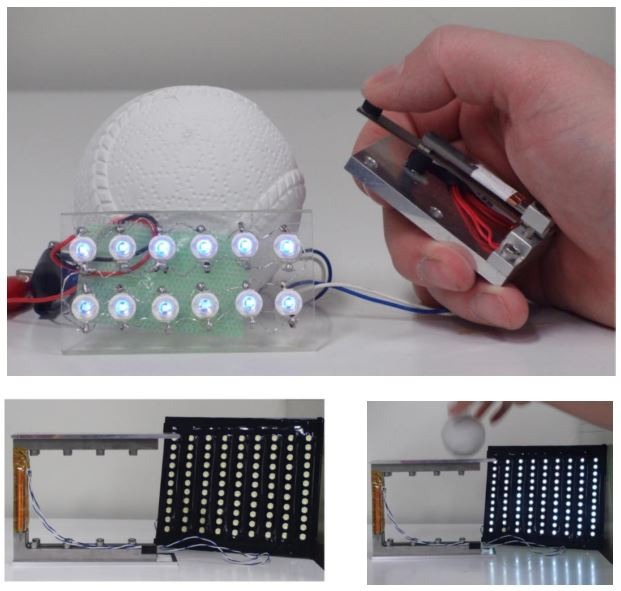
\includegraphics[trim=0pt 10pt 0pt 0pt,scale=0.5]{energy-harvest-demo}
	\caption{Galfenol resonant beam energy harvester. Photo courtesy of Dr. Toshiyuki Ueno, Kanazawa University, Japan. Galfenol beams are in the same region as the coils and have dimensions of 3 mm thick x 15 mm width x 80 mm length.\cite{Slaughter2011}}
	\label{fig:energy-harvest-demo}
\end{figure}
The iron-based magnetostrictive alloy Fe-Ga (Galfenol, \fegacomp) is of interest for actuation, sensing and energy harvesting applications because in addition to its magnetostrictive properties, it is ductile and it has robust mechanical properties\cite{Clark2003}, relatively high permeability and good saturation magnetization (~1.7 T)\cite{Clark2002}. These properties allow our collaborator at Kanazawa University, Toshiyuki Ueno, to prototype highly-scalable Galfenol energy harvester devices with high efficiency, high power output, and low impedance\cite{Ueno2015a}, as seen in Figure \ref{fig:energy-harvest-demo}. Fe-Al (Alfenol, \fealcomp) has been overlooked as an actuactor because it has about half the magnetostriction of Fe-Ga alloys. However, Fe-Al has similar saturation magnetization ($\sim$1.5 T) and similar mechanical properties to Fe-Ga, making it an attractive energy harvester with the added benefit of being more earth abundant and less expensive than Fe-Ga\cite{Na2014a,Raghunath2014a}. 		

Fe-Al is sufficiently magneto-elastic that coupling between bending stress and magnetic moment rotation yields readily observable time-varying magnetization changes in the alloy. In harvesters, power is generated in a copper coil that surrounds a magnetostrictive material when a time varying stress, e.g. vibration of the magnetostrictive material, produces a voltage in the coil (per Faraday’s law)\cite{Yoo2012}. Fe-Al is a body-centered cubic alloy textured to develop a  preferred orientation along the length of the strips by abnormal grain growth (AGG)\cite{Na2014,Na2014b,Na2013a}. The \hkl<100> directions are the magnetic easy axes. Subsequently, the stress annealing protocol was performed to introduce built-in uniaxial anisotropy perpendicular to the length of the strips\cite{Yoo2009}.  This was done to maximize 90$^{\circ}$ rotation of magnetic moments when the strip bends. Successful stress-anneal-induced magnetic anisotropy was achieved, but this stress annealing process could not provide uniform compressive stress on each tested sample leading to non-uniform magnetic flux change along the strip length. As a viable alternative for a uniform magnetic flux change, Brooks et al. have used magnetic field annealing to achieve nearly identical saturation magnetostriction under compressive and no preload values\cite{Brooks2012}. 

\begin{figure}[h]
	\centering
	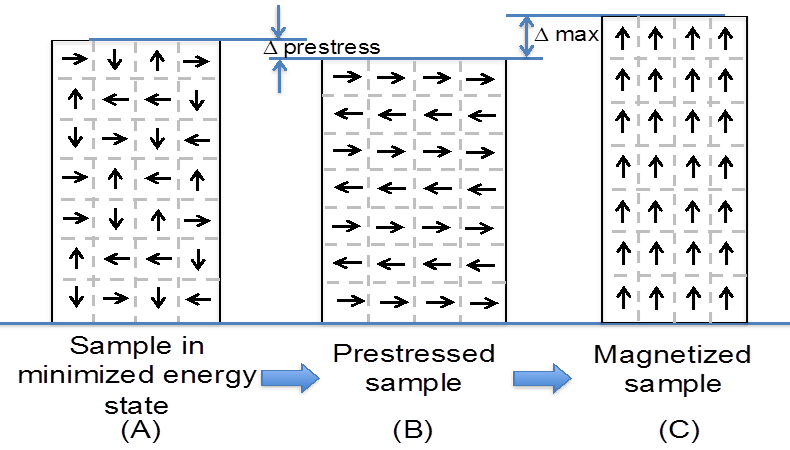
\includegraphics[trim=0pt 10pt 0pt 0pt,scale=0.5]{prestressed-mag-anneal}
	\caption{Cartoons depicting a perfectly aligned cubic alloy with \hkl<100> magnetic easy axes as indicated. Arrows depict idealized orientation of magnetic domains.(A) Energy minimized state with closure domains randomly distributed throughout sample.  (B) Prestressed sample with aligned antiparallel magnetization vectors and sample length minimized due to stress-induced moment rotation. (C) Sample magnetized along length with $\Delta$max as the maximum achievable magnetostriction due to 90~$^{\circ}$ magnetic moment rotation.}
	\label{fig:prestressed-mag-anneal}
\end{figure}




\subsection{Motivation}\label{abnormal-grain-growth}
%Describes Abnormal Grain Growth from Dr. Na's papers
%
\subsubsection{Process of AGG from Na2012 \cite{Na2012b} }
%TODO Edit in own words


Magnetostrictive Fe–Ga alloys (Galfenol) have promising attributes for application to sensors, actuators and energy harvesting as Clark et al. first reported in 2000\cite{clark2000magnetostrictive}. Single-crystal Galfenol has a body-centered
cubic (bcc) crystal structure, and along the \hkl<100> crystal orientations, it exhibits saturation magnetostriction of $\sim$400 ppm in low applied magnetic fields of $\sim$200 Oe. It also has a mechanical strength of $\sim$500 MPa, which is high relative to more costly rare earth magnetostrictive materials such as Terfenol-D alloys which exhibit giant magnetostriction ($\gtrsim$1600 ppm) but are brittle and require much higher magnetic fields ($\gtrsim$1000 Oe) for saturation\cite{clark2000magnetostrictive,Clark2003,Guruswamy2000}. The large magnetostriction and easy magnetization in single-crystal Galfenol alloys occur along the \hkl<100> orientation. It is thus desirable to obtain the \hkl<100> orientation in textured polycrystalline Galfenol, with the goal of providing enhanced mechanical properties and lower cost than single-crystal material, with similar magnetostrictive strain. 

Two viable approaches have been employed to fabricate highly textured Fe–Ga alloys\cite{srisukhumbowornchai2001large,kellogg2003texture}. One is a directional solidification growth process, and the other is thermomechanical processing involving deformation via rolling and recrystallization through grain growth and orientation mechanisms. Galfenol rods grown by the directional solidification process have strong crystallite textures with \hkl<100> preferred orientation aligned 14$^{\circ}$ off from the rod direction and a maximum magnetostriction ($\lambda_{\parallel}$) of 271 ppm under compression \cite{srisukhumbowornchai2001large}. In other works, Kellogg et al. reported that binary Fe$_{0.83}$Ga$_{0.17}$ with a somewhat dispersed \hkl{001}\hkl<100> texture along rolling direction (RD) exhibited magnetostrictive strain of $\sim$160 ppm as a consequence of rolling and annealing at 1100$^{\circ}$C for 4 h\cite{kellogg2003texture}. Texture annealing of Fe$_{0.85}$Ga$_{0.15}$ alloy with 1 mol.\% NbC at 1150–1300$^{\circ}$C for 24 h changed the texture from a strong $\alpha$-fiber texture \hkl<110>$\parallel$RD in as-rolled sheet to a preferred texture with \hkl<100> orientation\cite{srisukhumbowornchai2004crystallographic}. The authors did not report the magnetostriction values; however, an estimated of lower than 135 ppm can be made based on their electron backscatter diffraction (EBSD) data and the nominal saturation value in a single crystal with the same composition. In our prior work, we have demonstrated the texture development of Goss \hkl{011}\hkl<100> texture through secondary recrystallization by using NbC particles as an inhibitor of normal grain growth(NGG) \cite{Na2009}.

%TODO: Connect AGG to surface energy

\subsubsection{Need for Surface Energy}

\textbf{Galfenol} \\
\textbf{Galfenol AGG is affected by sulfur surface segregation concentration}

We have been studying the development of Goss- and Cube-textured Galfenol rolled sheet as a low-cost alternative to magnetostrictive single crystal Galfenol for several years. We targeted Goss and Cube textures to obtain one and two directions respectively of easy magnetic axes and high magnetostriction in the plane of the rolled sheet. An additional benefit of developing a Cube texture is that it will make feasible use magnetic field annealing to maximize performance\cite{Yoo2008,Yoo2009} and thereby eliminate the need for stress annealing or use of prestress components in the design of devices that use these materials.\cite{Restorff2006,Summers2009b} Developing protocols for making thin sheet Galfenol with Goss or Cube textures has been challenging because the mechanisms that regulate grain boundary mobility and texture development in these alloys are not well understood. The preliminary results in Fig. \ref{fig:AGG-diagram} show AGG and texture development in Galfenol rolled sheet for several different anneal protocols. The dramatic difference in AGG and texture between the result in the top right image and the results in the two lower right images was accomplished by building on empirical insights from studies of Fe and Fe-Si alloys in which control of surface energy was used to regulate grain growth and ultimately to produce Cube-textured material.\cite{Walter1965,dunn1962surface,waeckerle1993effect,Kramer1992}

In Fig. \ref{fig:AGG-diagram}, as-rolled polycrystalline Galfenol (left image) exhibits a strong $\gamma$-fiber and weak rotated cube textures, and starts with an $\alpha$-iron (B2) structure. A partly grown Goss texture developed over $\sim$39$\%$ of the sample surface area during a 3h argon-anneal (upper right image) due to grain boundary energy alone. We have also demonstrated that small variations in surface energy have a significant impact of the development of texture.\cite{Chun2010,Na2012b} The two lower right images show AGG with fully developed \hkl(001) and \hkl(011) grains over 90-95$ \% $ of the sample surface. AGG of (011) grains is very reproducible (insensitive to small variations in anneal conditions), while the development of (001) grains is challenging to produce/reproduce (highly sensitive to anneal conditions). Saturation magnetostriction values equal to 90$ \% $ and 84$ \% $ of single crystal \hkl(100) values for alloy of the same composition were measured in sulfur-annealed samples with \hkl(001) and \hkl(011) grain growth, respectively. Auxeticity of these samples has not been investigated. 

\begin{figure}[h] 
	\centering
	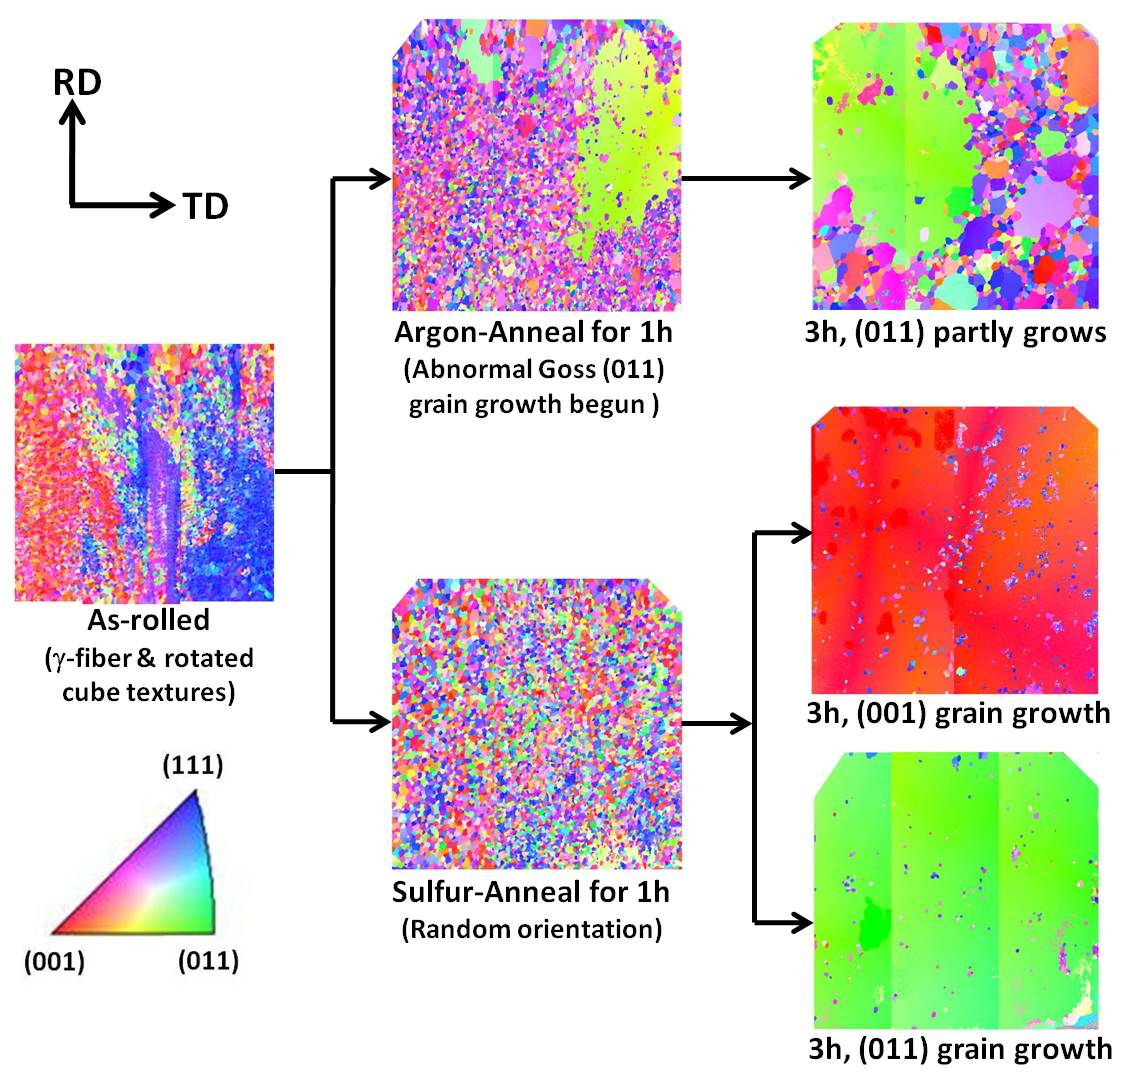
\includegraphics[width=0.7\textwidth]{AGG-diagram}
	\caption{Diagram of AGG from as-rolled sample of (Fe-19$\%$Ga)+1.0$\%$NbC alloy (left) to argon- (upper) and sulfur-annealed (lower) samples for annealing times of 1h (middle) and 3h (right). EBSD images scanned along the normal direction of 12x12x0.45 mm$^{3}$ sheet. Red, green and blue indicate \hkl(001), \hkl(011) and \hkl(111) grains, respectively. 
	}
	\label{fig:AGG-diagram}		
\end{figure}

Figure \ref{fig:AGG-diagram} results are the first and only that we know of to employ concepts that date back to the mid-1960’s \cite{Walter1965,dunn1962surface,waeckerle1993effect} for developing AGG in irons, Fe-Si and silicon-steels together with Kramer’s work in the 1990’s\cite{Kramer1992} on control of surface energy to develop Cube texture in Fe-Si. Our research hypothesis is motivated by our desire to understand the physical metallurgy that lead to these results and be able to routinely reproduce these results in rare-earth-free anisotropic alloys. \\
\textbf{Alfenol}

\textbf{Alfenol AGG is affected differently than Galfenol under sulfur concentrations. This must be due to the differences in orientation-dependent surface energy between Galfenol and Alfenol.}

%TODO Insert need for Alfenol surface energy from UMERC proposal. Want the Cube texture for easier magnetic annealing!

The importance of Alfenol surface energy lies in the Aerosmart Lab's need for more efficient energy harvesting materials, as discussed in Section \ref{magnetostrict-materials}. Currently, stress-annealed and field-annealed samples are first rolled into sheets from ingots, and then atmospherically annealed to develop large grains that cover over 90\% of the sample surface area. This process avoids lengthy and expensive single-crystal growth methods. We target Goss \hkl{110} and Cube \hkl{100} textures to obtain one and two directions, respectively, of easy magnetic axes and high magnetostriction in the plane of the rolled sheet. Goss-textured Alfenol can reach magnetostrictive constants of ~184 ppm, and the elusive Cube-textured Alfenol would reach even higher magnetostriction values due to the additional direction of easy magnetic axes. An added benefit of developing a Cube texture is that it will make feasible use of magnetic field annealing to maximize performance\cite{Yoo2009,Yoo2008} and thereby eliminate the need for stress annealing or use of pre-stress components in the design of devices that use these materials\cite{Restorff2006,Summers2009}.
	


 Magnetostrictive Fe–Ga alloys (Galfenol) have promising attributes for application to sensors, actuators and energy harvesting as Clark \etal first reported in 2000\cite{clark2000magnetostrictive}. Single-crystal Galfenol has a body-centered cubic (bcc) crystal structure, and along the \hkl<100> crystal orientations, it exhibits saturation magnetostriction of $\sim$400 ppm in low applied magnetic fields of $\sim$200 Oe. It also has a mechanical strength of $\sim$500 MPa, which is high relative to more costly rare earth magnetostrictive materials such as Terfenol-D alloys which exhibit giant magnetostriction ($\gtrsim$1600 ppm) but are brittle and require much higher magnetic fields ($\gtrsim$1000 Oe) for saturation\cite{clark2000magnetostrictive,Clark2003,Guruswamy2000}. The large magnetostriction and easy magnetization in single-crystal Galfenol alloys occur along the \hkl<100> orientation. It is thus desirable to obtain the \hkl<100> orientation in textured polycrystalline Galfenol, with the goal of providing enhanced mechanical properties and lower cost than single-crystal material, with similar magnetostrictive strain. 

%TODO: Insert paragraph about Alfenol properties and why they are good.
%TODO: CORRECTION -> will insert paragraph about Alfenol if necessary. 



 Two viable approaches have been employed to fabricate highly textured Fe–Ga alloys\cite{srisukhumbowornchai2001large,kellogg2003texture}. One is a directional solidification growth process, and the other is thermomechanical processing involving deformation via rolling and recrystallization through grain growth and  
\begin{figure}[h]
	\centering
	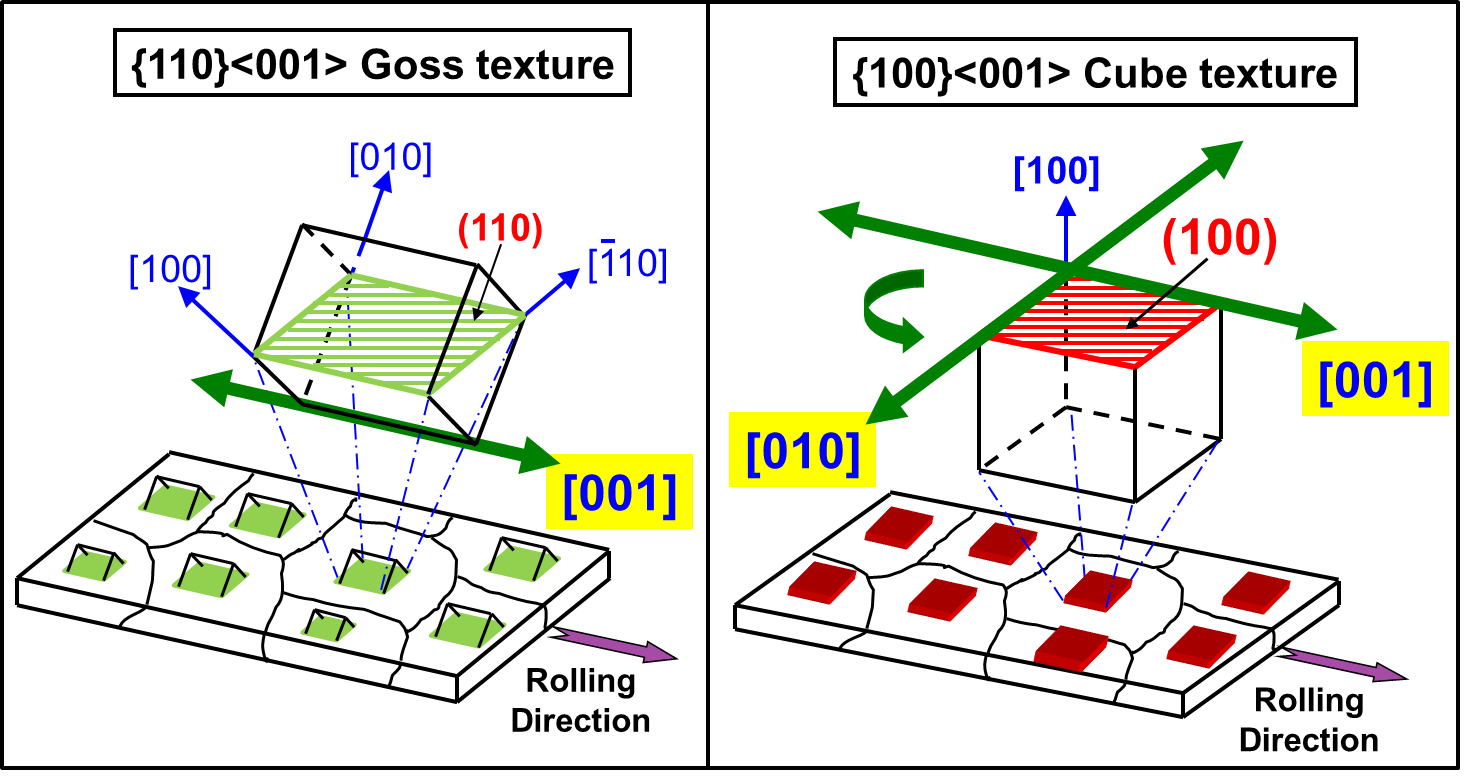
\includegraphics[width=0.8\textwidth,trim={0 0 0 0.5cm}]{goss_cube}
	\caption{Illustration of Goss and Cube textures shown with their respective axes of easy magnetization.}
	\label{fig:goss_cube}	
\end{figure}
 orientation mechanisms. Currently, stress-annealed and field-annealed samples are first rolled into sheets from ingots, and then atmospherically annealed to develop large grains on the sample surface area by utilizing the abnormal grain growth (AGG) phenomenon. 


 AGG is often detrimental in piezoelectric ceramics because it lowers the hardness and the larger developed grain sizes lead to degradation of the piezoelectric effect.\cite{Bing2014} For our application goals, we use AGG to our advantage by targeting Goss \hkl{110} and Cube \hkl{100} textures to obtain one and two directions, respectively, of easy magnetic axes and high magnetostriction in the plane of rolled sheets. This process avoids lengthy and expensive single-crystal growth methods while still producing Galfenol with sufficient magnetostrictive properties for device application. We have been studying the development of Goss- and Cube-textured Galfenol rolled sheet as a low-cost alternative to magnetostrictive single crystal Galfenol for several years. To optimize specific grain growth, we have  incorporated pinning particles during the rolling process, experimented with different annealing temperatures and times, and modified the annealing environment.\cite{Na2007b,Na2008,Na2009,Na2012} 

 EBSD images spatially map crystal orientations on well-polished specimen by using backscattered electron patterns from the electron beam in a scanning electron microscope (SEM). From these patterns, we can use statistical tools to measure average misorientation, grain size, and crystallographic texture. Fig. \ref{fig:AGG-diagram} depicts electron backscatter diffraction (EBSD) images of more successful annealing conditions we have tested. As-rolled polycrystalline Galfenol (left image) exhibits a strong $\gamma$-fiber and weak rotated cube textures, and starts with an $\alpha$-iron (B2) structure. A partly grown Goss texture developed over $\sim$39$\%$ of the sample surface area during a 3h argon-anneal (upper right image) due to grain boundary energy alone. This is because large inert argon particles only adsorb to the Galfenol surface, rather than penetrating the lattice and causing surface-energy-modifying segregation. We have also demonstrated that small variations in surface energy have a significant impact of the development of texture.\cite{Chun2010,Na2012b} The two lower right images show AGG with fully developed \hkl(001) and \hkl(011) grains over 90-95$ \% $ of the sample surface. 
\begin{wrapfigure}[14]{l}{0.5\linewidth}
	\centering
	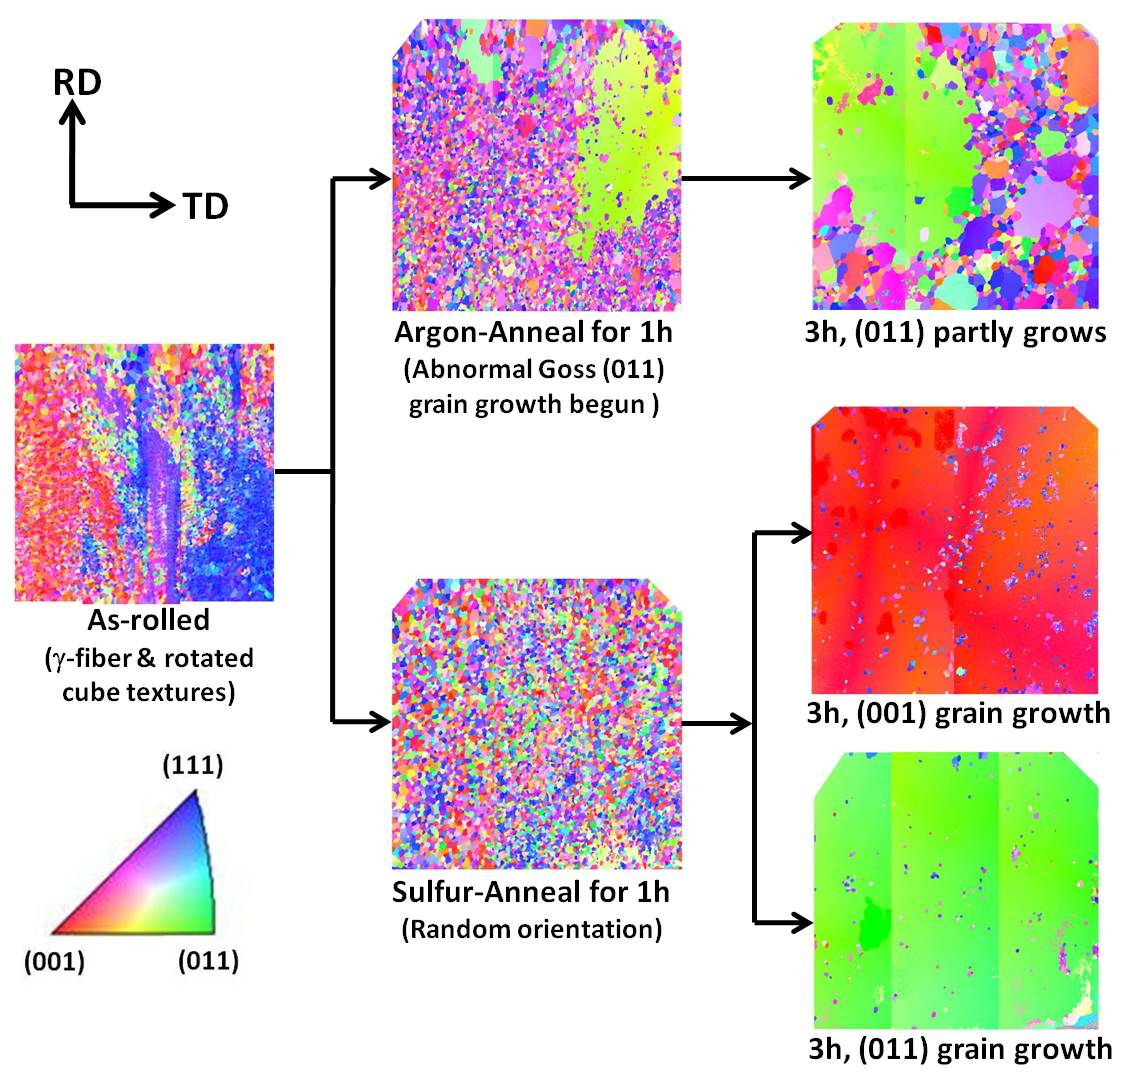
\includegraphics[width=0.45\textwidth,trim={0 0 0 0}]{AGG-diagram}
	\caption{Diagram of AGG from as-rolled sample of (Fe-19$\%$Ga)+1.0$\%$NbC alloy (left) to argon- (upper) and sulfur-annealed (lower) samples for annealing times of 1h (middle) and 3h (right). EBSD images scanned along the normal direction of 12x12x0.45 mm$^{3}$ sheet. Red, green and blue indicate \hkl(001), \hkl(011) and \hkl(111) grains, respectively. 
	}
	\label{fig:AGG-diagram}	
\end{wrapfigure}
 AGG of (011) grains is very reproducible (insensitive to small variations in anneal conditions), while the development of (001) grains is challenging to produce/reproduce (highly sensitive to anneal conditions). Saturation magnetostriction values equal to 90$ \% $ and 84$ \% $ of single crystal \hkl(100) values for alloy of the same composition were measured in sulfur-annealed samples with \hkl(001) and \hkl(011) grain growth, respectively.  

 Developing protocols for making thin sheet Galfenol with Goss or Cube textures has been challenging because the mechanisms that regulate grain boundary mobility and texture development in these alloys are not well understood. Modelling techniques that examine grain boundary interactions, coincident site lattice (CSL) and high energy grain boundary (HEGB), have been investigated to understand AGG mechanisms. These techniques were able to sufficiently describe abnormally grown Goss grains in \fegacomp(x=19)+1.0 mol\% NbC rolled sheets, but mechanisms for abnormally grown Cube-grains are still not known.\cite{Chun2010} We believe that these models are insufficient because they do not incorporate extraneous driving forces caused by the control of surface energy from atmospheric annealing conditions, as described by Kramer \etal By characterizing the surface energy of specific Galfenol grains, we can develop a more accurate thermodynamic-based framework for modeling AGG and texture development that will be used to understand why a high temperature atmospheric anneal transforms myriad crystallite grains into the highly textured, single-crystal-like polycrysalline material. 

%Figure \ref{fig:AGG-diagram} results are the first and only that we know of to employ concepts that date back to the mid-1960’s \cite{Walter1965,dunn1962surface,waeckerle1993effect} for developing AGG in irons, Fe-Si and silicon-steels together with Kramer’s work in the 1990’s\cite{Kramer1992} on control of surface energy to develop Cube texture in Fe-Si. Our research hypothesis is motivated by our desire to understand the physical metallurgy that lead to these results and be able to routinely reproduce these results in rare-earth-free anisotropic alloys. 



%\subsubsection{Need for Surface Energy}

%\textbf{Galfenol} 
%\textbf{Galfenol AGG is affected by sulfur surface segregation concentration}

 

%An additional benefit of developing a Cube texture is that it will make feasible use magnetic field annealing to maximize performance\cite{Yoo2008,Yoo2009} and thereby eliminate the need for stress annealing or use of prestress components in the design of devices that use these materials.\cite{Restorff2006,Summers2009b} The preliminary results in Fig. \ref{fig:AGG-diagram} show AGG and texture development in Galfenol rolled sheet for several different anneal protocols. The dramatic difference in abnormal grain growth (AGG) and texture between the result in the top right image and the results in the two lower right images was accomplished by building on empirical insights from studies of Fe and Fe-Si alloys in which control of surface energy was used to regulate grain growth and ultimately to produce Cube-textured material.\cite{Walter1965,dunn1962surface,waeckerle1993effect,Kramer1992}



%In other works, Kellogg et al. reported that binary Fe$_{0.83}$Ga$_{0.17}$ with a somewhat dispersed \hkl{001}\hkl<100> texture along rolling direction (RD) exhibited magnetostrictive strain of $\sim$160 ppm as a consequence of rolling and annealing at 1100$^{\circ}$C for 4 h\cite{kellogg2003texture}. Texture annealing of Fe$_{0.85}$Ga$_{0.15}$ alloy with 1 mol.\% NbC at 1150–1300$^{\circ}$C for 24 h changed the texture from a strong $\alpha$-fiber texture \hkl<110>$\parallel$RD in as-rolled sheet to a preferred texture with \hkl<100> orientation\cite{srisukhumbowornchai2004crystallographic}. In our prior work, we have demonstrated the texture development of Goss \hkl{011}\hkl<100> texture through secondary recrystallization by using NbC particles as an inhibitor of normal grain growth(NGG) \cite{Na2009}.


%\begin{figure}[h!] 
%	\centering
%	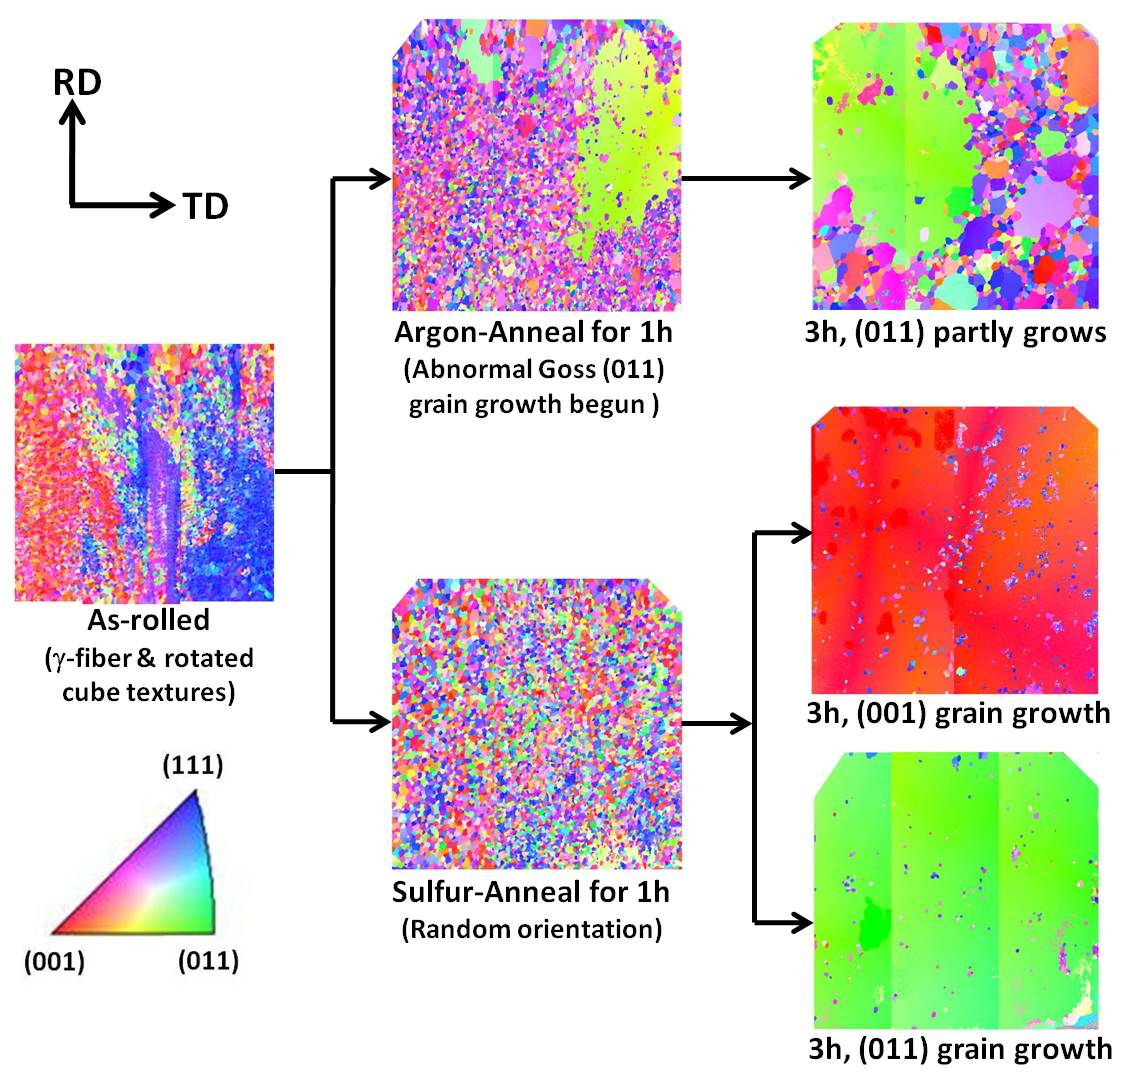
\includegraphics[width=0.6\textwidth]{AGG-diagram}
%	\caption{Diagram of AGG from as-rolled sample of (Fe-19$\%$Ga)+1.0$\%$NbC alloy (left) to argon- (upper) and sulfur-annealed (lower) samples for annealing times of 1h (middle) and 3h (right). EBSD images scanned along the normal direction of 12x12x0.45 mm$^{3}$ sheet. Red, green and blue indicate \hkl(001), \hkl(011) and \hkl(111) grains, respectively. 
%	}
%	\label{fig:AGG-diagram}		
%\end{figure}




%\textbf{Alfenol}

%TODO: Take this paragraph to the end as a future work thing. "This research has the potential for extension to other systems. Specifically, for ou
%The importance of Alfenol surface energy lies in the Aerosmart Lab's need for more efficient energy harvesting materials. Goss-textured Alfenol can reach magnetostrictive constants of ~184 ppm, and the elusive Cube-textured Alfenol would reach even higher magnetostriction values due to the additional direction of easy magnetic axes. An added benefit of developing a Cube texture is that it will make feasible use of magnetic field annealing to maximize performance\cite{Yoo2009,Yoo2008} and thereby eliminate the need for stress annealing or use of pre-stress components in the design of devices that use these materials\cite{Restorff2006,Summers2009}. Clearly, Alfenol AGG is affected differently than Galfenol under sulfur concentrations. This must be due to the differences in orientation-dependent surface energy between Galfenol and Alfenol.


%\subsection{Surface Energy}\label{surface-energy}

\subsubsection{Defining Surface Energy}\label{define-surf-energy}
%TODO: Rewrite entire section in your own words in order to not copyright the author below. 
%\textbf{Interface Science and Composites (Chapter 3: Solid-Liquid Interface), by Soo-Jin Park and Min-Kang Seo\cite{Park2011a}}


 Thermodynamically, the physical origin of the surface free energy is the excess Gibbs free energy of matter at the interface. Atoms or molecules exposed at an interface are surrounded by fewer neighbors, such as solid, liquid, and gas phases, resulting in an anisotropic distribution of these neighbors, which is the characteristic of a surface. Interaction energy must be shared between phases with the neighboring molecules. Hence, the surface free energy, $\gamma$, represents the rate of change of the Gibbs free energy of the system with respect to the area, $A$, at a constant pressure and temperature\cite{Chattoraj2012}:
\begin{equation}\label{SFE}
	\gamma = \left(\frac{\partial G}{\partial A}\right)_{T,P}
\end{equation}
 In principle, Equation \ref{SFE} can be used to calculate the surface tension of a condensed phase held together by the long-range forces. 

 The interaction of a liquid with a solid is characterized by the term "wetting." Wetting can be understood as the spreading of a liquid over a solid surface, the penetration of a liquid into porous materials, or the displacement of one liquid by another. This phenomenon can help to characterize a surface, and to determine the interaction between a solid and a liquid. 

 One way to quantify a liquid's surface wetting characteristics is to measure the contact angle of a drop of liquid placed on the surface of an object. The contact angle formed by the solid-liquid and liquid-vapor interfaces are measured from the side of the liquid. Liquids wet surfaces when the contact angle is less than 90\degree. For a penetrant material to be effective, the contact angle should be as small as possible. In fact, the contact angle for most liquid penetrants approach 0\degree. 

 The wetting ability of a liquid is a function of the surface energy of the solid-vapor interface, the liquid-gas interface, and the solid-liquid interface. The surface energy across an interface or the surface tension at the interface is a measure of the energy required to form the unit area of a new surface at the interface. The intermolecular bonds, or cohesive forces, between the molecules of a liquid cause surface tension. When the liquid encounters another substance, there is usually an attraction between the two materials. The adhesive forces between the liquid and the second substance will compete against the cohesive forces of the liquid.  Liquids with strong cohesive bonds and weaker adhesive forces will tend to bead-up or form a droplet when in contact with another material. Liquids with relatively weak cohesive bonds and a strong attraction to another material, or the desire to create adhesive bonds, will tend to spread over the material, such is the case with water droplets on high-surface energy metal substrates.
 
 \begin{wrapfigure}[8]{R}{0.5\linewidth}
 	\centering
 	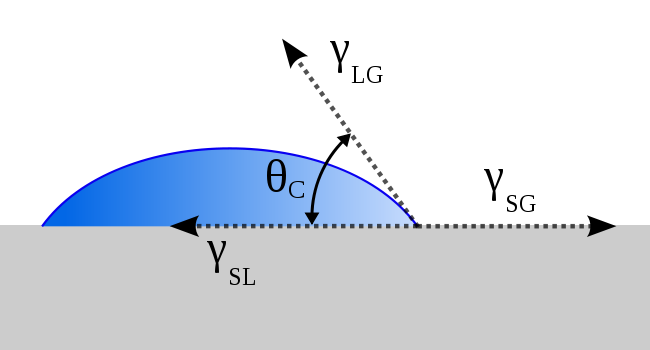
\includegraphics[width=0.5\textwidth,trim={0 0 0 2cm}]{Contact_angle}
 	\caption{This illustration shows a vector representation of the interfacial tensions involved in a solid-liquid-gas contact angle experiment. [Image available in public domain: wikimedia.org]}
 	\label{fig:ca-vector}
 \end{wrapfigure}

 Depending on the thermodynamic state or the hydrodynamic status of the liquid drop in which the contact angle is measured, two types of contact angels can be defined. If the contact angle is measured when either the liquid drop contines to spread or when its thermodynamic state conditions continue to change, the measured contact angle is termed the dynamic contact angle. However, if the contact angle is measured under conditions in which the liquid drop is stationary and the surrounding conditions in which the liquid drop is stationary and the surrounding conditions are in the steady state, the measured contact angle is known as the static/equilibrium contact angle. The contact angle technique is chosen for studies of the wettability phenomena owing to its simplicity. 


 The solid-liquid interface plays a fundamental role in diverse fields and helps with an understanding of physical phenomena and structural knowledge of the interface at the atomic scale. Fields of interest include catalysis, lubrication, electrochemistry, colloidal systems, biological reactions, and, most relevantly, crystal growth. Therefore, unravelling the atomic structure at the solid-liquid interface is one of the major challenges. 


 Contact angle measurements, as described by Thomas Young in 1805, remain the most accurate method for determining the interaction energy between a liquid (L) and a solid (S) in a condensed state at the minimum equilibrium distance of S and L. This is defined geometrically as the angle formed by a liquid at the three-phase boundary, where vapor, liquid, and solid intersect. It measures the result of liquid cohesion energy, $\gamma_{L}$ and the energy of adhesion between a liquid and solid. Young described the equilibrium contact angle at the three-phase boundary in terms of the vectorial sum, as shown in Figure \ref{fig:ca-vector}, resulting in an equilibrium force balance. The famous Young's equation is derived from the Gibbs free energy at equilibrium, as seen from the result of Equation \ref{young_eqn}. 


\hypertarget{youngeqn}{}
\begin{equation}\label{young_eqn}
	\boxed{\gamma_{SV} =\gamma_{SL}-\gamma_{LV}\cos\theta}	
\end{equation}
%\end{tcolorbox}
 %We attempt to model a new contact angle method based on Equation \ref{young_eqn} in Section \ref{section2}

\subsection{Preliminary investigations}
There are currently no experimental methods available to measure surface energies associated with different crystallographic orientations of metals. High temperature methods involving cylindrical metal samples and destructive methods involving drop shape samples of a targeted liquid metal near the melting point are available for measuring surface energy of amorphous and isotropic solid metals.\cite{Egry2010,Aqra2011,Cao2011} For our research, however, we require knowledge of orientation-, morphology- and composition-dependent surface energies for validation of DFT results and for use in abnormal grain growth simulations. For glass and polymeric solids with relatively low surface energies, the water-drop method has been shown to be effective for the determination of surface energy at room temperature.\cite{Ahadian2010,Kwok2000,Tavana2005} We attempted to use this approach for contact angle measurements on large 17.9$\%$Ga Galfenol single crystal samples with \hkl(001), \hkl(011) and \hkl(111) grains with facilities at NIST. Results from this experiment were inconclusive because a large range of \ca[s] were measured for each single-crystal surface. This was most likely due to oxidation on the Galfenol surface causing a non-ideal, non-pristine surface. These results are also inconsistent with the predicted outcome of water completely wetting the high-energy surface, which may be a result of the sample roughness. While each sample may have been polished using silica gel with 60 nm particles,\cite{Costa2016} there could have been enough roughness at the droplet location to trap the triple-phase boundary and cause higher \ca[s] than expected. 

\subsubsection{Thermal Grooving}

The thermal grooving technique was briefly examined to potentially enlighten interactions between adjacent grains in Galfenol that we target for AGG. EBSD identified grain orientations on samples of Galfenol to identify the grain boundaries where \hkl(100), \hkl(110), and \hkl(111) orientations met. By measuring the dihedral angle formed at these grain boundaries, the ratio of grain boundary energy and surface energy was calculated according to the following equation: 
\begin{equation}
\frac{\gamma_{GB}}{\gamma_{S}} = 2\cos\left(\frac{\Psi_{S}}{2}\right) 
\end{equation}
where $\gamma_{GB}$ is the grain boundary energy, $\gamma_{S}  $ is the surface energy, and $\Psi_{S} $ is the dihedral angle, as described in Rohrer \etal\cite{Rohrer2010a} The most symmetric thermal groove came from a \hkl(110)/\hkl(111) grain boundary on a rolled and annealed (Fe-19\%Ga)+1.0\%NbC sample made 
\begin{figure}[h!]
	\centering
	\begin{subfigure}[c]{0.45\textwidth}
		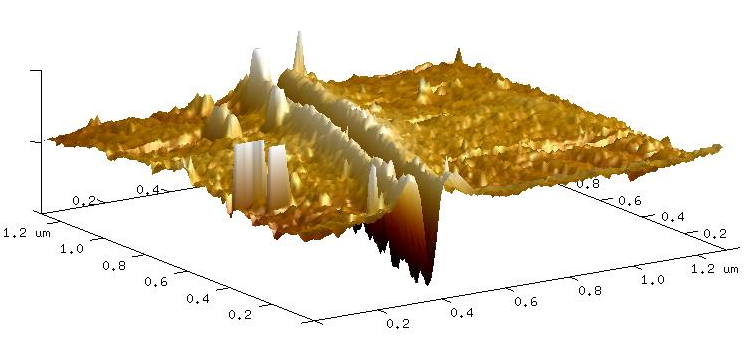
\includegraphics[width=\linewidth]{afm-groove-fega}
		\subcaption{~}
		\label{fig:afm-groove-fega}		
	\end{subfigure}
	\begin{subfigure}[c]{0.45\textwidth} 
		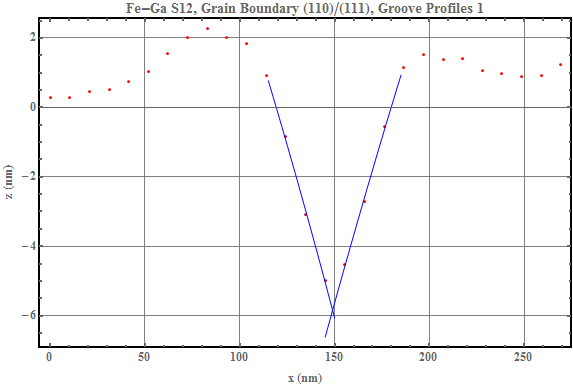
\includegraphics[width=\linewidth]{fega-groove-profile}
		\subcaption{~}
		\label{fig:fega-groove-profile}		
	\end{subfigure}
	\caption{(a) 3D rendering of (110)/(111) grain boundary on surface of  for (Fe-19\%Ga)+1.0\%NbC sample where the depth of groove is ~8 nm. (b) A quadratic fit of a (110)/(111) grain boundary profile for a (Fe-19\%Ga)+1.0\%NbC sample.}
	\label{fig:thermal-groove}
\end{figure}
by Suok-Min Na, as seen in the Figure \ref{fig:thermal-groove}.  The grain boundary profiles were measured using atomic force microscopy (AFM), and the dihedral angles were extrapolated from the profiles using both AFM software by Bruker and a quadratic fit.  The results are shown in Table \ref{groove-analysis}. This groove in particular had a depth of $\sim$8 nm which is significantly smaller in depth compared to grooves of other metal alloys.\cite{Skidmore2004a} Relative energies between 1/4 and 1/2 are expected for metals, but this small groove might explain why we see high variation in dihedral angles on the same groove. Many of the grain boundary grooves were not suitable for measuring based on their lack of symmetry at the grain boundary interface. To properly analyze the thermal grooving technique, an extensive grain boundary study of annealing temperatures and times on Galfenol would need to be investigated. While this may be an interesting avenue of research in the future, the resultant calculations of relative grain energies does not benefit our ultimate goal of achieving a comprehensive AGG model for Galfenol. Realization of this project's goal lies in the measurement of orientation-dependent surface energy using contact angle measurements. 


\begin{table}[h!]
	\centering
	\caption{Calculated dihedral angles and relative energies from our most symmetric grain boundary groove.}
	\begin{tabular} { |p{1cm}||c|c|c|c|  } 
		\hline
		\multicolumn{5}{|c|}{fe-ga-s12-006 profile analysis - GB (110)/(111)}\\
		\hline
		~	&\multicolumn{2}{|c|}{Bruker Software}		&\multicolumn{2}{|c|}{Quadratic Fit}	\\
		\hline
		Profile	&Dihedral Angle (\degree)	&Relative Energy	&Dihedral Angle (\degree)	&Relative Energy \\ 
		\hline
		1		&156.957	&0.399471	&151.253	&0.496475	\\
		\hline
		2		&156.244	&0.411657	&157.093	&0.397144	\\
		\hline
		3		&154.402	&0.443063	&155.554	&0.423432	\\
		\hline
		4		&157.221	&0.394955	&152.785	&0.470541	\\
		\hline
		5		&154.732	&0.437445	&154.966	&0.433458	\\
		\hline
		6		&158.386	&0.375003	&154.482	&0.441706	\\
		\hline
		\textbf{Avg}	&156.324~$\pm$1.529	&0.410266 $\pm$0.0261178	&154.356 $\pm$2.069	&0.443793 $\pm$0.0351932\\
		\hline
	\end{tabular}
	\label{groove-analysis}
\end{table}

%\subsubsection{Defining Surface Energy}
\textbf{Interface Science and Composites (Chapter 3: Solid-Liquid Interface), by Soo-Jin Park and Min-Kang Seo\cite{Park2011a}}

Thermodynamically, the physical origin of the surface free energy is the excess Gibbs free energy of the matter at the interface. Atoms or molecules exposed at an interface are surrounded by fewer neighbors, such a solid, liquid, and gas phases, resulting in an anisotropic distribution of these neighbors, which is the characteristic of a surface. They must share some of the the interaction energy with the neighboring molecules. Hence, the surface free energy, $\gamma$, represents the rate of change of the Gibbs free energy of the system with respect to the area, $A$, at a constant pressure and temperature\cite{Chattoraj2012}:
\begin{equation}\label{SFE}
	\gamma = \left(\frac{\partial G}{\partial A}\right)_{T,P}
\end{equation}
In principle, Equation \ref{SFE} can be used to calculate the surface tension of a condensed phase held together by the long-range forces. 

The interaction of a liquid with a solid is characterized by the word "wetting." It can be the spreading of a liquid over a solid surface, the penetration of a liquid into porous materials, or the displacement of one liquid by another. This phenomenon can help to characterize a surface, and to determine the interaction, between a solid and a liquid. 

One way to quantify a liquid's surface wetting characteristics is to measure the contact angle of a drop of liquid placed on the surface of an object. The contact angle formed by the solid-liquid interface and the liquid-vapor interface measured from the side of the liquid. Liquids wet surfaces when the contact angle is less than 90\degree. For a penetrant material to be effective, the contact angle should be as small as possible. In fact, the contact angle for most liquid penetrants is very close to 0\degree. 

The wetting ability of a liquid is a function of the surface energy of the solid-vapor interface, the liquid-gas interface, and teh solid-liquid interface. The surface energy across an interface or the surface tension at the interface is a measure of the energy required to form the unit area of a new surface at the interface. The intermolecular bonds or cohesive forces between the molecules of a liquid cause surface tension. When the liquid encounters another substance, there is usually an attraction between the two materials. The adhesive forces between the liquid and the second substance will compete against the cohesive forces of the liquid. Liquids with weak cohesive bonds and a strong attraction to another material (or the desire to create adhesive bonds) will tend to spread over the material. Liquids with strong cohesive bonds and weaker adhesive forces will tend to bead-up or form a droplet when in contact with another material. 

Depending on the thermodynamic state or the hydrodynamic status of the liquid drop in which the contact angle is measured, two types of contact angels can be defined. If the contact angle is measured when either the liquid drop contines to spread or when its thermodynamic state conditions continue to change, the measured contact angle is termed the dynamic contact angle. However, if the contact angle is measured under conditions in which the liquid drop is stationary and the surrounding conditions in which the liquid drop is stationary and the surrounding conditions are in the steady state, the measured contact angle is known as the static/equilibrium contact angle. The contact angle technique is chosen for studies of the wettability phenomena owing to its simplicity. 

The solid-liquid interface plays a fundamental role in diverse fields and helps with an understanding of physical phenomena and structural knowledge of the interface at the atomic scale. Fields of interest include catalysis, lubrication, electrochemistry, colloidal systems, biological reactions, and, most relevantly, crystal growth. Therefore, unravelling the atomic structure at the solid-liquid interface is one of the major challenges. 

\begin{outline}[enumerate]
	\1 Derivation of Young's Equation\\
	Assuming an ideally flat surface
	\begin{equation} \label{dropvol}
	V_{drop} = \frac{\pi R^{3}}{3} (1-\cos\theta)^{2} (2+\cos\theta)
	\end{equation}
	\begin{equation} \label{liqvapSA}
	S_{LV} = 2\pi R^{2} (1-\cos\theta)
	\end{equation}
	
	Where $S_{LV}$ is the surface area of the droplet liquid-vapor interface. The Gibbs free energy of a droplet is depicted in Equation \ref{liqvapSA}.
	
	\begin{equation} \label{gibbsdroplet}
	G = \gamma_{LV} S_{LV} + \pi(R \sin\theta)^{2} (\gamma_{SL}-\gamma_{SV})\\
	\end{equation}
	
	Let $a = \gamma_{SL}-\gamma_{SV}$. 
	
	Assuming the the volume of the droplet remains constant:
	\begin{equation*}
	\begin{gathered}
	G = \left[\frac{9\pi V^{2}}{(1-\cos\theta)(2+\cos\theta)^{2}}\right]^{2/3}
	\left[2\gamma_{LV} - a(1+\cos\theta)\right]\\
	\frac{dG}{d\theta} = \left[\frac{9\pi V^{2}}{(1-\cos\theta)^{4}(2+\cos\theta)^{5}}\right]^{1/3}
	2\left[a-\gamma_{LV}\cos\theta)\right]\sin\theta\\ \\
	\begin{split}
	\left[\frac{dG}{d\theta}\right]_{\theta=\theta_{eq}}&=0=a-\gamma_{LV}\cos\theta\\
	\therefore a 	&= \gamma_{LV}\cos\theta\\
	\end{split}					
	\end{gathered}
	\end{equation*}
	\begin{equation}\label{youngs-eqn}
	\boxed{\gamma_{SV} =\gamma_{SL}-\gamma_{LV}\cos\theta}	
	\end{equation}
\end{outline}

\subsubsection{\textbf{Insula}}
Surfaces have energy associated with them because work is needed to form them. Surface energy is the work per unit area done by the force that creates the new surface.

In the bulk, atoms are evenly surrounded and the cohesive forces between the atoms tend to balance. On the surface there are atoms on one side only, so there is a net inward cohesive force. This creates a force on the surface that tries to minimise its area. When considered as a force rather than an energy, the force is called "surface tension".

As temperature increases, the atoms in a solid vibrate more, and reduce the cohesive force binding the atoms. The surface energy depends on the net inward cohesive force and so surface energy decreases with increasing temperature. The surface energy for many metals (e.g. Ag, Au, and Cu) goes down by about 0.5 mJ/(m$^{2}\cdot K$) with increasing temperature. Water goes down by about 160 mJ/(m$^{2}\cdot K$).

\subsubsection{\textbf{Wikipedia}}
%TODO: Find citations from this snippet
The energy of the bulk component of a solid substrate is determined by the types of interactions that hold the substrate together. High energy substrates are held together by bonds, while low energy substrates are held together by forces. Covalent, ionic, and metallic bonds are much stronger than forces such as van der Waals and hydrogen bonding. High energy substrates are more easily wet than low energy substrates.[5] In addition, more complete wetting will occur if the substrate has a much higher surface energy than the liquid.[6]

Many techniques can be used to enhance wetting. Surface treatments (such as Corona treatment and acid etching) can be used to increase the surface energy of the substrate.[7][8] Additives can also be added to the liquid to decrease its surface energy. This technique is employed often in paint formulations to ensure that they will be evenly spread on a surface.[9]


